\subsection{Experimental Setup}
\label{sec:setup}

We employ a server equipped with two Intel Xeon Gold 6226R processors, each featuring $16$ cores running at a clock speed of $2.90$ GHz. Every core is equipped with a $1$ MB L1 cache, a $16$ MB L2 cache, and shares a $22$ MB L3 cache. The system has $93.4$ GB of memory and runs on CentOS Stream 8. We use GCC 8.5 and OpenMP 4.5. Table \ref{tab:dataset} displays the graphs utilized in our experiments, all sourced from the SuiteSparse Matrix Collection \cite{suite19}.

\begin{table}[hbtp]
  \centering
  \caption{List of $13$ graphs obtained SuiteSparse Matrix Collection \cite{suite19} (directed graphs are marked with $*$). Here, $|V|$ is the number of vertices, $|E|$ is the number of edges (after adding reverse edges), $D_{avg}$ is the average degree, and $|\Gamma|$ is the number of communities obtained using LPA.\ignore{In the table, B refers to a billion, M refers to a million and K refers a thousand.}}
  \label{tab:dataset}
  \begin{tabular}{|c||c|c|c|c|}
    \toprule
    \textbf{Graph} &
    \textbf{\textbf{$|V|$}} &
    \textbf{\textbf{$|E|$}} &
    \textbf{\textbf{$D_{avg}$}} &
    \textbf{\textbf{$|\Gamma|$}} \\
    % \textbf{$1 - \Gamma_G$} \\
    \midrule
    \multicolumn{5}{|c|}{\textbf{Web Graphs (LAW)}} \\ \hline
    indochina-2004$^*$ & 7.41M & 341M & 41.0 & 4.24K \\ \hline  % & \num{4.7e-4} & 2.9 GB
    uk-2002$^*$ & 18.5M & 567M & 16.1 & 42.8K \\ \hline  % & \num{9.6e-5} & 16 GB
    arabic-2005$^*$ & 22.7M & 1.21B & 28.2 & 3.66K \\ \hline  % & \num{5.5e-4} & 11 GB
    uk-2005$^*$ & 39.5M & 1.73B & 23.7 & 20.8K \\ \hline  % & \num{9.6e-5} & 16 GB
    webbase-2001$^*$ & 118M & 1.89B & 8.6 & 2.76M \\ \hline  % & \num{7.3e-7} & 18 GB
    it-2004$^*$ & 41.3M & 2.19B & 27.9 & 5.28K \\ \hline  % & \num{3.8e-4} & 19 GB
    sk-2005$^*$ & 50.6M & 3.80B & 38.5 & 3.47K \\ \hline  % & \num{5.8e-4} & 33 GB
    \multicolumn{5}{|c|}{\textbf{Social Networks (SNAP)}} \\ \hline
    com-LiveJournal & 4.00M & 69.4M & 17.4 & 2.54K \\ \hline  % & \num{7.9e-4} & 480 MB
    com-Orkut & 3.07M & 234M & 76.2 & 29 \\ \hline  % & \num{6.7e-2} & 1.7 GB
    \multicolumn{5}{|c|}{\textbf{Road Networks (DIMACS10)}} \\ \hline
    asia\_osm & 12.0M & 25.4M & 2.1 & 2.38K \\ \hline  % & \num{8.4e-4} & 200 MB
    europe\_osm & 50.9M & 108M & 2.1 & 3.05K \\ \hline  % & \num{6.6e-4} & 910 MB
    \multicolumn{5}{|c|}{\textbf{Protein k-mer Graphs (GenBank)}} \\ \hline
    kmer\_A2a & 171M & 361M & 2.1 & 21.2K \\ \hline  % & \num{9.4e-5} & 3.2 GB
    kmer\_V1r & 214M & 465M & 2.2 & 6.17K \\ \hline  % & \num{3.2e-4} & 4.2 GB
  \bottomrule
  \end{tabular}
\end{table}
% We convert directed graphs (marked with $*$) to undirected by duplicating edges in the reverse direction, and set the weight of each edge to $1$. and $F_{size}$ is size of the \textit{MatrixMarket} file

\begin{figure*}[hbtp]
  \centering
  \subfigure[Runtime in seconds (logarithmic scale) with \textit{FLPA}, \textit{igraph LPA}, \textit{NetworKit LPA}, and \textit{GVE-LPA}]{
    \label{fig:rak-compare--runtime}
    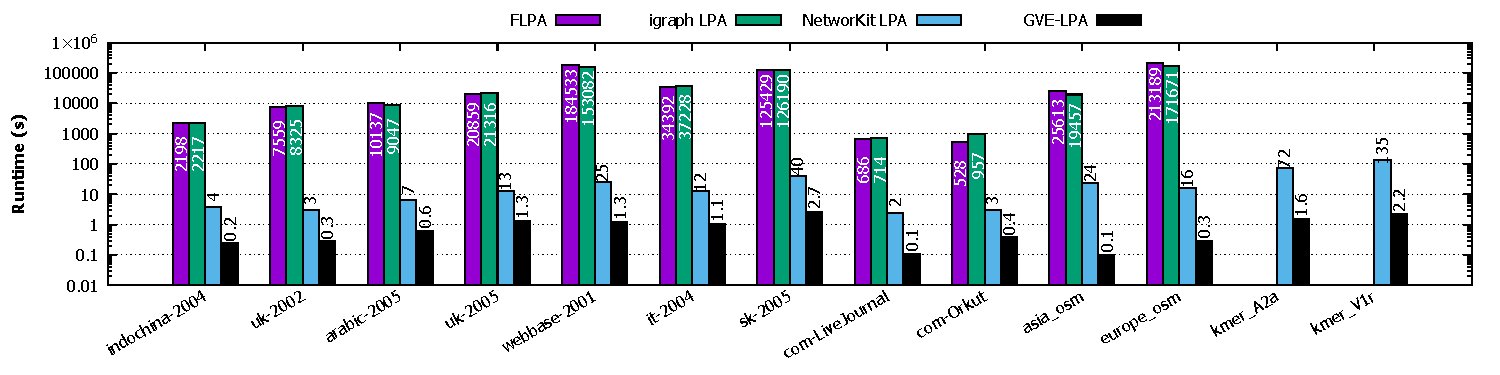
\includegraphics[width=0.98\linewidth]{out/rak-runtime.pdf}
  } \\[-0ex]
  \subfigure[Speedup (logarithmic scale) of \textit{GVE-LPA} with respect to \textit{FLPA}, \textit{igraph LPA}, \textit{NetworKit LPA}.]{
    \label{fig:rak-compare--speedup}
    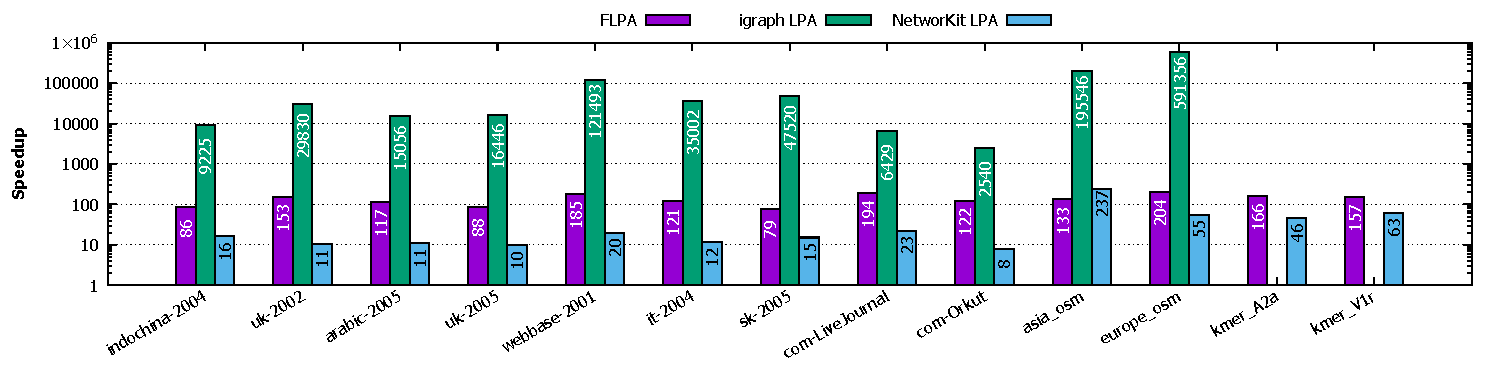
\includegraphics[width=0.98\linewidth]{out/rak-speedup.pdf}
  } \\[-0ex]
  \subfigure[Modularity of communities obtained with \textit{FLPA}, \textit{igraph LPA}, \textit{NetworKit LPA}, and \textit{GVE-LPA}.]{
    \label{fig:rak-compare--modularity}
    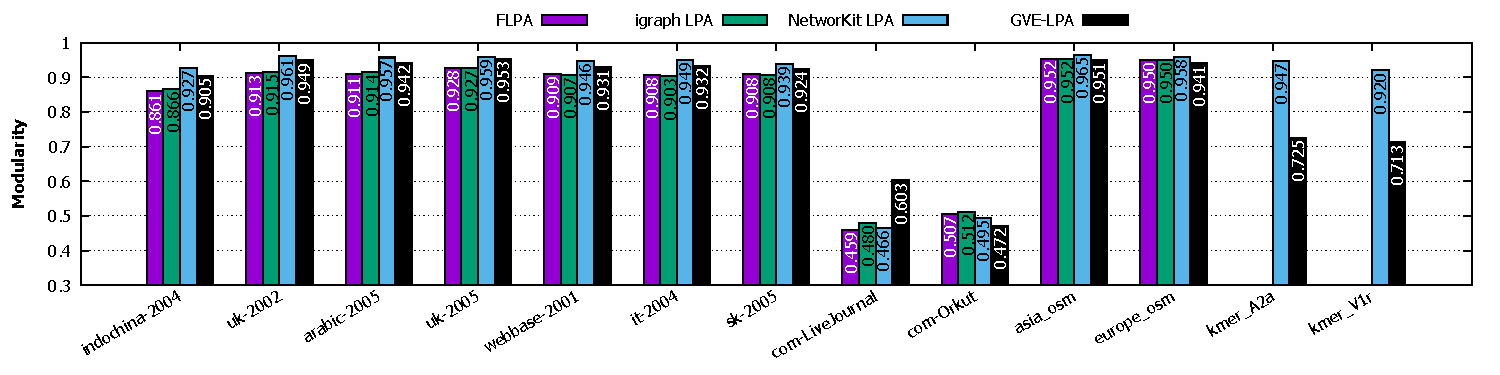
\includegraphics[width=0.98\linewidth]{out/rak-modularity.pdf}
  } \\[-2ex]
  \caption{Runtime\ignore{in seconds (logarithmic scale)}, speedup, and modularity of communities obtained with \textit{FLPA}, \textit{igraph LPA}, \textit{NetworKit LPA}, and \textit{GVE-LPA} for each graph\ignore{in the dataset}. \textit{FLPA} and \textit{igraph LPA} fail to run on \textit{kmer\_A2a} and \textit{kmer\_V1r} graphs, and thus their results are not shown.}
  \label{fig:rak-compare}
\end{figure*}

\begin{figure*}[hbtp]
  \centering
  \subfigure[Runtime in seconds (logarithmic scale) with \textit{GVE-Louvain} and \textit{GVE-LPA}]{
    \label{fig:louvainrak-compare--runtime}
    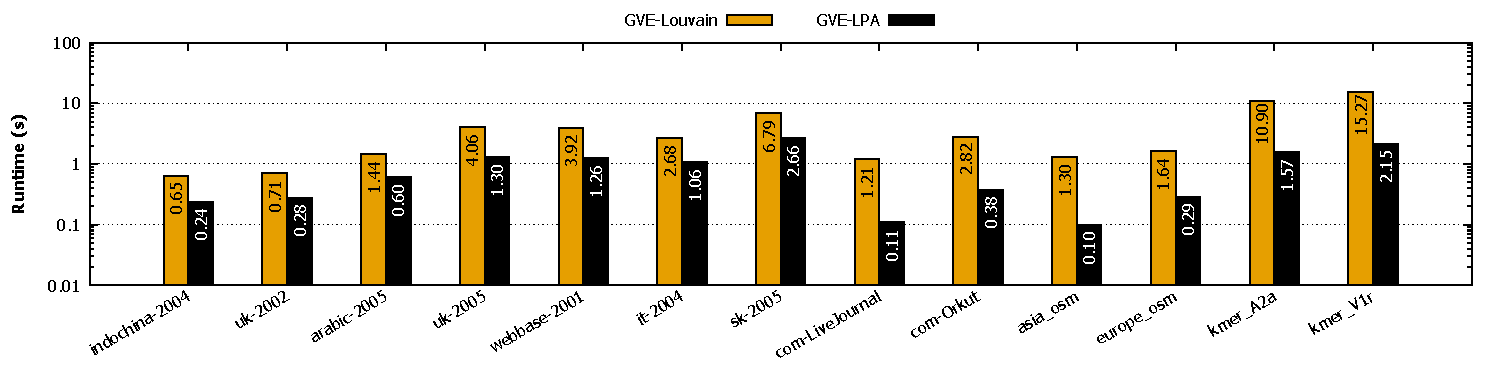
\includegraphics[width=0.98\linewidth]{out/louvainrak-runtime.pdf}
  } \\[-0ex]
  \subfigure[Speedup of \textit{GVE-LPA} with respect to \textit{GVE-Louvain}.]{
    \label{fig:louvainrak-compare--speedup}
    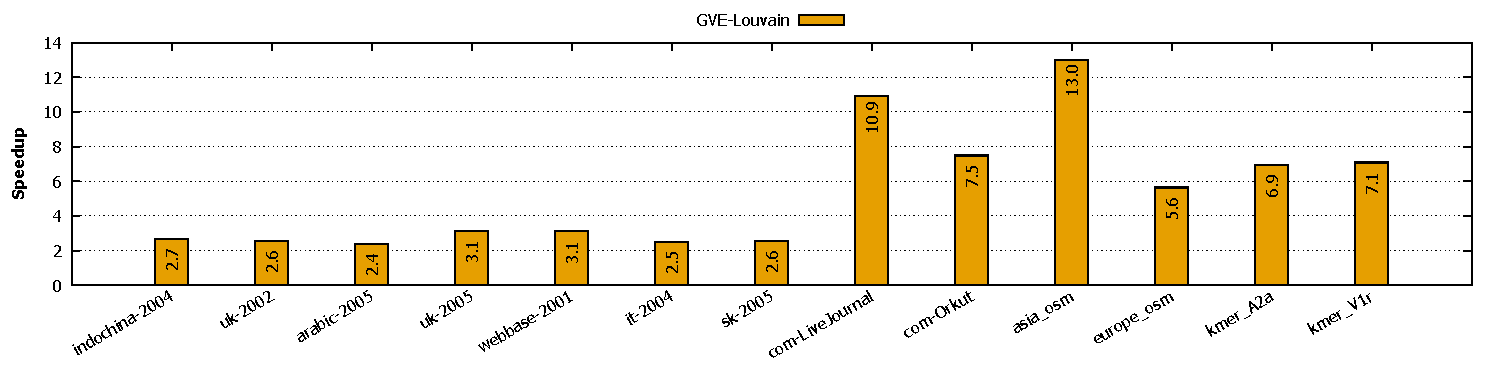
\includegraphics[width=0.98\linewidth]{out/louvainrak-speedup.pdf}
  } \\[-0ex]
  \subfigure[Modularity of communities obtained with \textit{GVE-Louvain} and \textit{GVE-LPA}.]{
    \label{fig:louvainrak-compare--modularity}
    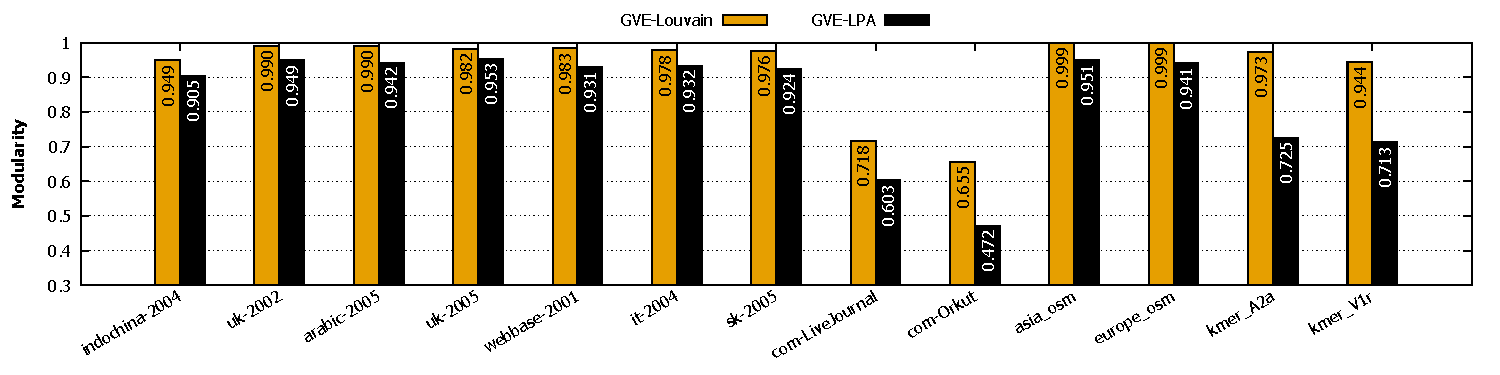
\includegraphics[width=0.98\linewidth]{out/louvainrak-modularity.pdf}
  } \\[-2ex]
  \caption{Runtime in seconds (logarithmic scale), speedup, and modularity of communities obtained with \textit{GVE-Louvain} \cite{sahu2023gvelouvain} and \textit{GVE-LPA} for each graph in the dataset.}
  \label{fig:louvainrak-compare}
\end{figure*}





\subsection{Comparing Performance of GVE-LPA}

We now compare the performance of GVE-LPA with FLPA \cite{traag2023large}, igraph LPA \cite{csardi2006igraph}, and NetworKit LPA \cite{staudt2016networkit}. FLPA and igraph LPA are both sequential implementations, while NetworKit LPA is parallel. For FLPA, we checkout the suitable branch with modified \texttt{igraph\_community\_label\_propagation()} function, update the label propagation example in C to load the input graph from a file and measure runtime of \texttt{igraph\_community\_label\_propagation} \texttt{()} with \texttt{gettimeofday()}. For igraph LPA, we follow a similar process as FLPA, but checkout code from the \texttt{master} branch of igraph. For NetworKit, we employ a Python script to invoke \texttt{PLP} (Parallel Label Propagation), and measure the total time reported with \texttt{getTiming()}. For each graph, we measure the NetworKit LPA runtime five times for averaging. Due to time constraints and long running times of FLPA and igraph LPA, we ran them only once per graph. Additionally, we record the modularity of communities obtained from each implementation.

Figure \ref{fig:rak-compare--runtime} shows the runtimes of FLPA, igraph LPA, NetworKit LPA, and GVE-LPA for each graph in the dataset, while Figure \ref{fig:rak-compare--speedup} shows the speedup of GVE-LPA with respect to each aforementioned implementation. Both FLPA and igraph LPA fail to run on \textit{kmer\_A2a} and \textit{kmer\_V1r} graphs, and hence their results are not shown. GVE-LPA exhibits an average speedup of $97,000\times$, $118,000\times$, and $40\times$ over FLPA, igraph LPA, and NetworKit LPA, respectively, especially on road networks and protein k-mer graphs with low average degrees. On the \textit{sk-2005} graph, GVE-LPA identifies communities in $2.7$ seconds, achieving a processing rate of $1.4$ billion edges/s. Figure \ref{fig:rak-compare--modularity} shows the modularity of communities obtained by each implementation. On average, GVE-LPA obtains $0.6\%$ / $0.2\%$ higher modularity than FLPA and igraph LPA respectively (especially on web graphs), and $4.1\%$ lower modularity than NetworKit LPA (especially on protein k-mer graphs with large number of vertices and a low average degree).

\begin{figure}[hbtp]
  \centering
  \subfigure{
    \label{fig:rak-hardness--all}
    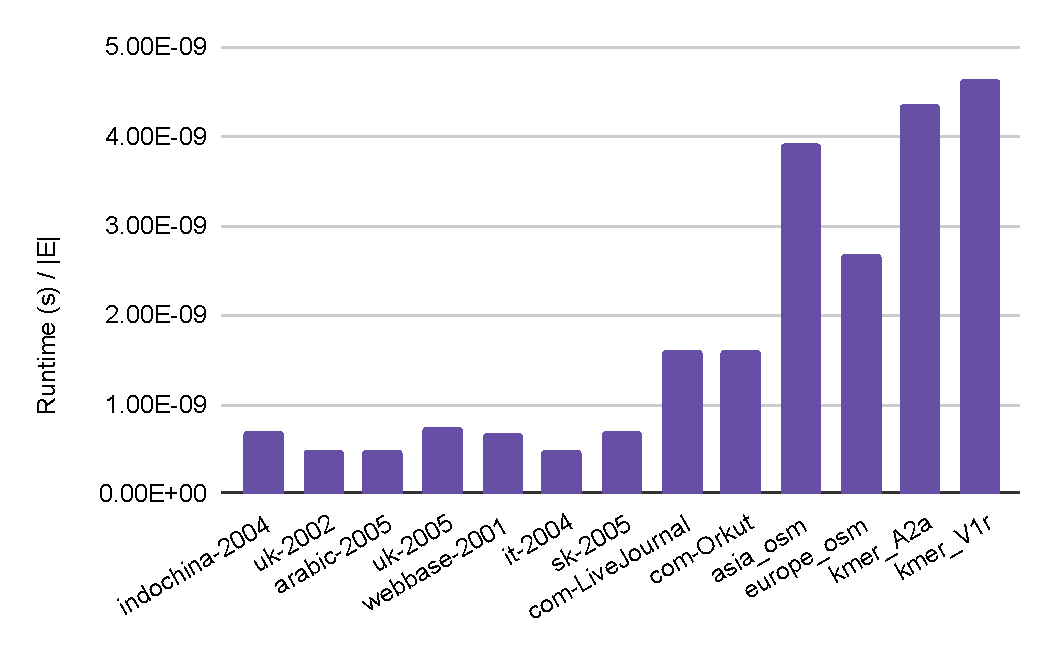
\includegraphics[width=0.98\linewidth]{out/rak-hardness.pdf}
  } \\[-2ex]
  \caption{Runtime $/ |E|$ factor with \textit{GVE-LPA} for each graph in the dataset.}
  \label{fig:rak-hardness}
\end{figure}

\begin{figure}[hbtp]
  \centering
  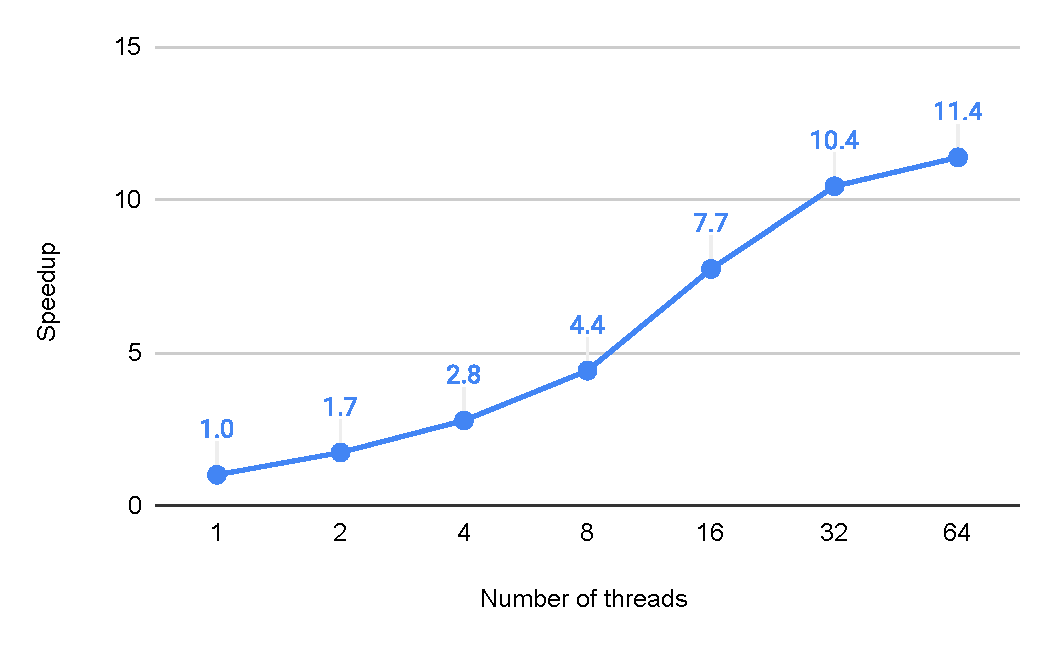
\includegraphics[width=0.98\linewidth]{out/rak-ss.pdf} \\[0ex]
  \caption{Average speedup of \textit{GVE-LPA} with increasing number of threads (in multiples of 2).}
  \label{fig:rak-ss}
\end{figure}


Next, we proceed to compare the performance of GVE-LPA with GVE-Louvain in Figure \ref{fig:louvainrak-compare}. Figures \ref{fig:louvainrak-compare--runtime}, \ref{fig:louvainrak-compare--speedup}, and \ref{fig:louvainrak-compare--modularity} present the runtimes, speedup (of GVE-LPA with respect to GVE-Louvain), and modularity of GVE-Louvain and GVE-LPA for each graph in the dataset. GVE-LPA offers a mean speedup of $5.4\times$ compared to GVE-Louvain, particularly on social networks, road networks, and protein k-mer graphs, while achieving on average $10.9\%$ lower modularity, especially on social networks and protein k-mer graphs.

In Figure \ref{fig:rak-hardness}, we assess the runtime per edge of GVE-LPA. Results indicate that GVE-LPA exhibits a higher $\text{runtime}/|E|$ factor on graphs with a low average degree (road networks and protein k-mer graphs) and on graphs with a poor community structure (\textit{com-LiveJournal} and \textit{com-Orkut}).




\subsection{Strong Scaling of GVE-LPA}

Finally, we assess the strong scaling performance of GVE-LPA. To this end, we vary the number of threads from $1$ to $64$ in multiples of $2$ for each input graph, and measure the time required for GVE-LPA to identify communities (averaged over five runs). Figure \ref{fig:rak-ss} shows the average strong-scaling of of GVE-LPA, in comparison with GVE-Louvain. With 32 threads, GVE-LPA achieves a speedup of $13.5\times$ compared to single-threaded execution, indicating a performance increase of $1.7\times$ for each doubling of threads. At 64 threads, GVE-LPA is moderately impacted by NUMA effects, and offers a speedup of $18.1\times$. This contrasts with GVE-Louvain, which appears to be significantly affected by NUMA effects.
